\hypertarget{ux5927ux8bedux8a00ux6a21ux578bux7684ux57faux672cux539fux7406}{%
\chapter{大语言模型的基本原理}\label{ux5927ux8bedux8a00ux6a21ux578bux7684ux57faux672cux539fux7406}}

\hypertarget{gptux4e0eux9884ux8badux7ec3}{%
\section{GPT与预训练}\label{gptux4e0eux9884ux8badux7ec3}}

\hypertarget{ux4e00ux6838ux5fc3ux601dux60f3-5}{%
\subsection{一、核心思想}\label{ux4e00ux6838ux5fc3ux601dux60f3-5}}

GPT（Generative Pre-trained Transformer）的核心思想是``预测 next token''，这是一个单向、自回归的生成过程。比如，第一次根据已有提示词，预测第一个 token（记为 \(x_1\)）；第二次根据提示词和 \(x_1\)，预测第二个 token \(x_2\)；第三次根据提示词和 \(x_1\)、\(x_2\)，预测第三个 token \(x_3\)\ldots\ldots 这样做的背后逻辑在于：一个真正强大的语言模型，仅仅通过``预测下一个词''这个任务，就能学到关于语言、知识、推理和思维的几乎所有规律。当模型的规模（参数、数据、算力）足够大时，这个看似简单的任务会迫使模型构建一个极其复杂和精确的对世界的模型，以便做出更好的预测。这个训练过程称为``预训练''（Pre-training），以和后续的微调（后训练）相区分。

事实上，这样的模型训练过程相当于将丰富的对世界的认识``压缩''在了模型参数中。有观点认为``压缩即智能''，因为为了在生成过程中获得高置信度的还原，模型必须从海量知识中提炼出内在规律，在训练时尽可能接近``无损压缩''。而这个提炼的过程也会让模型发现人类可能无法发现的一些不同领域知识间的内在关联，这也是创新的源泉之一（所以我们不能武断地认为 AI 不能创新）。当然，强化微调（后面会提到）也是 AI 能产生新策略的一个重要原因。

另外特别说明，这里的 GPT 指的是``生成式预训练 Transformer''这样一个通用架构，而并非特指 OpenAI 的 ChatGPT 系列模型（当然 ChatGPT 作为首个生成式 AI 产品，应该就是因这样的架构而命名的）。

\hypertarget{ux4e8cux6a21ux578bux67b6ux6784-1}{%
\subsection{二、模型架构}\label{ux4e8cux6a21ux578bux67b6ux6784-1}}

GPT 和 BERT 一样基于 Transformer，但和 BERT 不同的是，GPT 选用了 Transformer 架构的解码器部分，在三个注意力块中也只选用了其中的带掩码的多头自注意力（Masked Multi-Head Self-Attention）。

在这个注意力块中，查询、键、值均来自同一序列的已生成部分，每个词只能关注到它左边的词（即过去的词），而不能关注到它右边（即未来）的词，这决定了 GPT 的``单向性''。这是通过一个注意力掩码来实现的，它将未来位置的信息全部遮盖掉，确保模型在生成下一个词时，不会``偷看''到未来的答案，这与模型在推理时（生成模式）的行为保持一致。

GPT 模型由多层 Transformer 解码器块堆叠而成。例如，GPT-3 有 96 层。每个解码器块内部都包含一个全连接前馈网络，用于对每个位置的表示进行非线性变换。

为什么选择解码器？解码器的自回归特性天然契合``下一个词预测''的预训练任务。模型在训练时和推理时的行为是完全一致的，都是根据已知文本来预测未知文本，这避免了 BERT 存在的预训练-微调不一致问题。

\hypertarget{ux4e09ux4e3aux4ec0ux4e48ux4e0dux9700ux8981ux7f16ux7801ux5668ux4e3aux4ec0ux4e48ux6548ux679cux6bd4ux57faux4e8eux7f16ux7801ux5668ux7684-bert-ux66f4ux597d}{%
\subsection{三、为什么不需要编码器\&为什么效果比基于编码器的 BERT 更好？}\label{ux4e09ux4e3aux4ec0ux4e48ux4e0dux9700ux8981ux7f16ux7801ux5668ux4e3aux4ec0ux4e48ux6548ux679cux6bd4ux57faux4e8eux7f16ux7801ux5668ux7684-bert-ux66f4ux597d}}

\hypertarget{ux751fux6210ux80fdux529bux662fux66f4ux6839ux672cux66f4ux901aux7528ux7684ux80fdux529b}{%
\subsubsection{1. 生成能力是更根本、更通用的能力}\label{ux751fux6210ux80fdux529bux662fux66f4ux6839ux672cux66f4ux901aux7528ux7684ux80fdux529b}}

理解是生成的子集：要想高质量地生成一段文本，模型必须深刻地理解语言、知识、逻辑和上下文。一个能和你流畅对话的模型，其理解能力必然不差。反之，一个只擅长理解的模型（如 BERT），却无法进行流畅的生成。而通过``生成''范式，GPT 可以被引导去完成几乎任何 NLP 任务，这被称为``提示工程''。这种统一性使得一个模型可以应对千变万化的任务，而 BERT 通常需要为每个任务设计特定的模型结构和微调过程。

\hypertarget{scaling-law}{%
\subsubsection{2. Scaling Law}\label{scaling-law}}

大量实验发现，纯解码器的 Transformer 架构在当模型参数规模、数据量和计算力扩大到一定程度时，模型会涌现出令人惊讶的新能力（如推理、代码生成、复杂指令跟随等）。

当参数达到千亿级别（如 GPT-3）时，纯解码器架构涌现出了强大的上下文学习能力。这意味着，仅仅通过一个提示（Prompt），模型就能理解并执行各种复杂任务，而无需一个专门的编码器来为其解析指令。

这最终证明：一个足够庞大的自回归模型，其解码器本身就已经具备了我们期望编码器拥有的``深度理解''能力。它通过在生成过程中``反复咀嚼''前文，同样可以完成深度的语义理解。

\hypertarget{ux9884ux8badux7ec3ux4e0eux4f7fux7528ux4efbux52a1ux7684ux4e00ux81f4ux6027}{%
\subsubsection{3. 预训练与使用任务的一致性}\label{ux9884ux8badux7ec3ux4e0eux4f7fux7528ux4efbux52a1ux7684ux4e00ux81f4ux6027}}

GPT 的训练任务是下一个词预测（自回归），GPT 的推理/使用方式也是生成下一个词，并将其作为新的输入，继续生成下一个词（自回归）。模型在训练时和部署时的行为是完全一致的。它永远不会在训练时看到整个句子（因为未来词被掩码遮住了），在推理时也不需要看到未来词。这种一致性使得模型能够将其在训练中学到的所有能力，毫无损耗地应用到实际生成中。

反之，如果 GPT 在预训练时使用了编码器（双向注意力）来理解输入，那么在推理生成时就会遇到一个悖论：在生成第 \(N\) 个词时，编码器需要看到完整的输入序列才能进行编码，但完整的输入序列包含了尚未生成的未来词。因此，为了保持极致的任务一致性，抛弃编码器是必然的选择。

而训练过程与生成任务的不一致性也被认为是制约 BERT 性能（尤其是生成方面性能）的瓶颈之一。

\hypertarget{ux7f16ux7801ux5668ux7684ux5197ux4f59ux6027}{%
\subsubsection{4. 编码器的冗余性}\label{ux7f16ux7801ux5668ux7684ux5197ux4f59ux6027}}

编码器-解码器架构是为序列到序列任务设计的，比如机器翻译、文本摘要。这些任务的特点是输入和输出可以是不同长度、不同模态的，编码器要理解、编码整个输入序列（双向），再由解码器负责根据编码器的输出，自回归地生成输出序列，而 GPT 的任务更像是``文本续写''，而不是``文本转换''。

从参数和计算效率上，只训练一个解码器栈，相比训练编码器和解码器两个栈，在参数量相同的情况下，每个组件可以更``深''或更``宽''，模型能力可能更强。训练和推理过程也更简单，避免了编码器和解码器之间的复杂交互。

一个比喻：编码器-解码器（如 T5）像是一个翻译团队。编码器是分析源语言的研究员（全面理解原文），解码器是根据研究员报告撰写目标语言的作家（生成译文）；纯解码器（如 GPT）像是一个独自创作的作家。他一边阅读自己已经写下的前文（这本身就是``理解''过程），一边续写后面的内容。他不需要一个独立的研究员来告诉他前文是什么意思，因为他自己就是作者。

\hypertarget{ux6587ux672cux81eaux8eabux7684ux5e8fux5217ux6027}{%
\subsubsection{5. 文本自身的序列性}\label{ux6587ux672cux81eaux8eabux7684ux5e8fux5217ux6027}}

BERT 为代表的编码器架构在模型规模极大时，可能不如自回归的解码器有效，因为它破坏了文本的天然序列性。

\hypertarget{ux56dbux591aux6a21ux6001}{%
\subsection{四、多模态}\label{ux56dbux591aux6a21ux6001}}

多模态技术，就是让 AI 从单纯的``文字处理者''进化为具备``眼耳口脑''的全能感知体。它打破了文本、图像、音频和视频之间的壁垒，能够像人类一样同时通过看图、听声音和读文字来理解世界；例如，你不仅可以用文字提问，还能直接上传一段视频或一张图表让 AI 分析其中的逻辑。

目前主流的实现方法是通过一些方式，将各个模态的信息``对齐''到统一的高维语义空间中进行处理，从而在预训练中融合多个模态的数据。无论输入的是文本、图像还是音频，输入信息经过不同方式处理后，最终都会统一到同一个高维语义空间中。比如，``猫''这个词语和一张猫的图片在这个语义空间中距离较近，和一张西瓜的图片在空间中距离较远。具体实现方式可见多模态部分介绍。

\hypertarget{ux53c2ux8003ux6587ux732e-71}{%
\subsection{参考文献}\label{ux53c2ux8003ux6587ux732e-71}}

\begin{itemize}
\tightlist
\item
  Vaswani, A., Shazeer, N., Parmar, N., et al.~(2017). \href{https://arxiv.org/abs/1706.03762}{Attention Is All You Need}. NeurIPS 2017.
\item
  Radford, A., Narasimhan, K., Salimans, T., \& Sutskever, I. (2018). \href{https://cdn.openai.com/research-covers/language-unsupervised/language_understanding_paper.pdf}{Improving Language Understanding by Generative Pre-Training}. OpenAI.
\item
  Radford, A., Wu, J., Child, R., et al.~(2019). \href{https://cdn.openai.com/better-language-models/language_models_are_unsupervised_multitask_learners.pdf}{Language Models are Unsupervised Multitask Learners}. OpenAI.
\item
  Brown, T. B., Mann, B., Ryder, N., et al.~(2020). \href{https://arxiv.org/abs/2005.14165}{Language Models are Few-Shot Learners}. NeurIPS 2020.
\end{itemize}

\clearpage

\hypertarget{ux8bcdux5d4cux5165embedding}{%
\section{词嵌入（Embedding）}\label{ux8bcdux5d4cux5165embedding}}

\hypertarget{ux4e00ux8bcdux5d4cux5165embeddingux7684ux6574ux4f53ux6d41ux7a0b}{%
\subsection{一、词嵌入（Embedding）的整体流程}\label{ux4e00ux8bcdux5d4cux5165embeddingux7684ux6574ux4f53ux6d41ux7a0b}}

Tokenizer（分词器）把句子切分成词（Token），然后去词表里查出每个词对应的整数ID。词嵌入层（Embedding Layer）接收Tokenizer输出的整数ID，并将其转化为包含语义的浮点数向量，供后续的Attention层进行处理。

\hypertarget{ux4e8ctokenizerux5206ux8bcdux5668}{%
\subsection{二、Tokenizer（分词器）}\label{ux4e8ctokenizerux5206ux8bcdux5668}}

输入一个原始文本字符串，如``The cat sat''。Tokenizer先将字符串分解为``词元''(Token)，再根据一个在训练前就构建好的、从``词''到``ID''的映射字典，每个 Token 转换为其对应的整数 ID。如{[}``the'', ``cat'', ``sat''{]}转化为{[}2, 3, 4{]}，不是训练的对象。

\hypertarget{ux4e09embedding-layerux8bcdux5d4cux5165ux5c42}{%
\subsection{三、Embedding Layer（词嵌入层）}\label{ux4e09embedding-layerux8bcdux5d4cux5165ux5c42}}

它是神经网络内部的第一个层，输入是Tokenizer输出的整数ID序列，如{[}2, 3, 4{]}，输出这些ID对应的向量拼接成的矩阵。在数学上，这个过程可以用矩阵线性计算（无激活函数）表示。它的参数是每个Token的embedding向量表示，例如词汇表有 50,000 个词，每个词是一个300维向量，那这一层的参数量就是15,000,000。训练时根据输入和输出更新参数，通过参数的正确收敛（每个词嵌入向量能有效表达语义），实现对输入文段的正确输出表示。测试时，根据前向计算，得出每个Token的ID对应的嵌入向量。例如算出代表 ``the'' 的 300 维向量为{[}0.12, -0.45, \ldots, 0.88{]} ，代表 ``cat'' 的{[}0.67, 0.01, \ldots, -0.23{]}，代表 ``sat'' 的{[}-0.11, 0.98, \ldots, 0.51{]} ，输出{[}{[}0.12, \ldots{]}, {[}0.67, \ldots{]}, {[}-0.11, \ldots{]}{]}。

例如句子 \texttt{Don\textquotesingle{}t\ you\ love\ {[}emoji{]}\ Transformers?\ We\ sure\ do.} 在不同分词器下会得到不同的 Token 序列和 ID 序列：

\begin{itemize}
\tightlist
\item
  根据空格分词：\texttt{{[}"Don\textquotesingle{}t",\ "you",\ "love",\ "{[}emoji{]}",\ "Transformers?",\ "We",\ "sure",\ "do."{]}}，对应的 ID 序列为 \texttt{{[}1347,\ 249,\ 890,\ 1310,\ 8219,\ 568,\ 909,\ 791{]}}。
\item
  根据 spaCy 分词器分词：\texttt{{[}"Do",\ "n\textquotesingle{}t",\ "you",\ "love",\ "{[}emoji{]}",\ "Transformers",\ "?",\ "We",\ "sure",\ "do",\ "."{]}}，对应的 ID 序列为 \texttt{{[}91,\ 8123,\ 21313,\ 3123,\ 41251,\ 151,\ 9859,\ 115,\ 1515,\ 3134,\ 4114{]}}。
\end{itemize}

\hypertarget{ux53c2ux8003ux6587ux732e-72}{%
\subsection{参考文献}\label{ux53c2ux8003ux6587ux732e-72}}

\begin{itemize}
\tightlist
\item
  Vaswani, A., Shazeer, N., Parmar, N., et al.~(2017). \href{https://arxiv.org/abs/1706.03762}{Attention Is All You Need}. NeurIPS 2017.
\item
  Radford, A., Narasimhan, K., Salimans, T., \& Sutskever, I. (2018). \href{https://cdn.openai.com/research-covers/language-unsupervised/language_understanding_paper.pdf}{Improving Language Understanding by Generative Pre-Training}. OpenAI.
\end{itemize}

\clearpage

\hypertarget{ux751fux6210ux8fc7ux7a0bux7684ux5e72ux9884}{%
\section{生成过程的干预}\label{ux751fux6210ux8fc7ux7a0bux7684ux5e72ux9884}}

\hypertarget{ux4e00ux6e29ux5ea6temperature}{%
\subsection{一、温度（Temperature）}\label{ux4e00ux6e29ux5ea6temperature}}

\begin{itemize}
\tightlist
\item
  \textbf{高温值（如 1.0）}：增加生成结果的多样性，但可能导致结果不稳定。
\item
  \textbf{低温值（如 0.1）}：生成结果更稳定，但可能缺乏创造性。
\end{itemize}

温度参数控制生成结果的随机性。具体来说，温度参数 \(T\) 影响概率分布的``尖锐度''。温度越高，概率分布越平滑，生成结果的多样性越高；温度越低，概率分布越尖锐，生成结果越稳定。

\[
P(x_{T+1} \mid x_1, x_2, \ldots, x_T) =
\frac{\exp\left(\frac{f(x_1,x_2,\ldots,x_T)}{T}\right)}
{\sum_i \exp\left(\frac{f_i(x_1,x_2,\ldots,x_T)}{T}\right)}
\]

其中，\(f(x_1,x_2,\ldots,x_T)\) 是模型的内部函数，通常是一个复杂的神经网络，如 Transformer 架构。\(T\) 是温度参数，控制概率分布的平滑程度。

\hypertarget{ux4e8cux91c7ux6837ux641cux7d22ux8bcdux5143ux7b56ux7565}{%
\subsection{二、采样（搜索词元）策略}\label{ux4e8cux91c7ux6837ux641cux7d22ux8bcdux5143ux7b56ux7565}}

\hypertarget{ux8d2aux5fc3ux641cux7d22}{%
\subsubsection{贪心搜索}\label{ux8d2aux5fc3ux641cux7d22}}

始终选择概率最高的下一个词，生成结果稳定但可能单调。

\[
x_{T+1} = \arg\max P(x_{T+1} \mid x_1, x_2, \ldots, x_T)
\]

贪心搜索示例：图片展示了一个树状图，从 ``The'' 开始，每一步都选择概率最高的分支，例如 The -\textgreater{} nice (0.5) -\textgreater{} woman (0.4) \ldots{}

\begin{figure}[htbp]
\centering
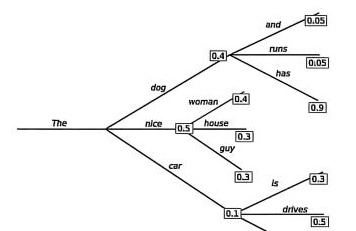
\includegraphics{images/image-0017.jpeg}
\caption{贪心搜索树状示例}
\end{figure}

问题：每步取最高≠乘积最高！

\hypertarget{ux6ce2ux675fux641cux7d22}{%
\subsubsection{波束搜索}\label{ux6ce2ux675fux641cux7d22}}

波束搜索通过在每个时间步保留最可能的 \texttt{num\_beams} 个词，并从中最终选择出概率最高的序列，来降低丢失潜在高概率序列的风险。

波束搜索示例：图片展示了树状搜索过程。与贪心搜索不同，它在每一步会保留多个路径，例如 ``The nice'' 和 ``The dog''，然后继续扩展。

\begin{figure}[htbp]
\centering
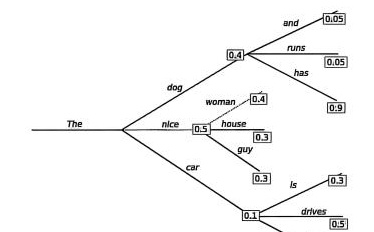
\includegraphics{images/image-0018.jpeg}
\caption{波束搜索树状示例}
\end{figure}

\textbf{Top-k 采样}：从概率最高的 \(k\) 个词中随机选择下一个词，平衡稳定性和多样性。

\[
S_k = \{x_i \mid P(x_i \mid x_1, x_2, \ldots, x_T) \mathcjk{ \mathcjk{是前} } k \mathcjk{ \mathcjk{高的}}\}
\]

\[
x_{T+1} \sim P(x_{T+1} \mid x_1, x_2, \ldots, x_T) \mathcjk{，\mathcjk{在} } S_k \mathcjk{ \mathcjk{中随机选择}}
\]

\textbf{Top-p 采样（Nucleus Sampling）}：从概率累积达到 \(p\) 的最小词集中随机选择下一个词，动态调整采样范围。

\[
S_p = \{x_i \mid \sum_{j=1}^{i} P(x_j \mid x_1, x_2, \ldots, x_T) \le p\}
\]

\[
x_{T+1} \sim P(x_{T+1} \mid x_1, x_2, \ldots, x_T) \mathcjk{，\mathcjk{在} } S_p \mathcjk{ \mathcjk{中随机选择}}
\]

下面是Top-p采样的示意图：

\begin{figure}[htbp]
\centering
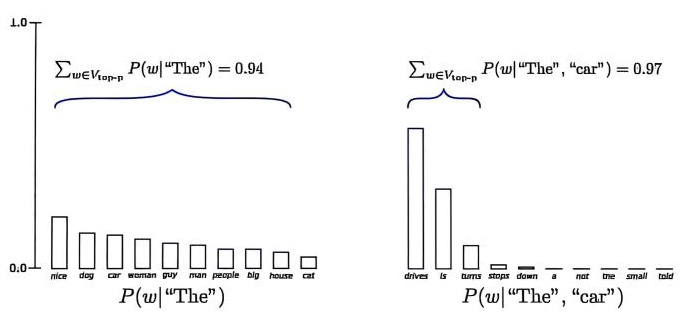
\includegraphics{images/image-0019.jpeg}
\caption{Top-p 采样分布示意图}
\end{figure}

也可以将Top-k与Top-p结合：先选K个，再从中选概率p。

\hypertarget{ux53c2ux8003ux6587ux732e-73}{%
\subsection{参考文献}\label{ux53c2ux8003ux6587ux732e-73}}

\begin{itemize}
\tightlist
\item
  《动手学大模型智能体》。
\end{itemize}

\clearpage

\hypertarget{ux540eux8badux7ec3}{%
\section{后训练}\label{ux540eux8badux7ec3}}

尽管预训练后的模型通过文本（或者还包括了其他类型的数据）学习到了海量的知识，但这样训练完毕的模型往往还不能满足人类的真实需求。大模型往往还需要经过后训练，即迁移学习（Transfer Learning）。具体地来说，就是要将一个在``源任务''（Source Task）上预训练好的模型所学到的知识，``迁移''并应用到一个新的、但相关的``目标任务''（Target Task）上。

\hypertarget{ux4e00ux4e3aux4ec0ux4e48ux8fc1ux79fbux5b66ux4e60ux5982ux6b64ux91cdux8981}{%
\subsection{一、为什么迁移学习如此重要？}\label{ux4e00ux4e3aux4ec0ux4e48ux8fc1ux79fbux5b66ux4e60ux5982ux6b64ux91cdux8981}}

迁移学习的出现是为了解决传统机器学习面临的两个核心挑战：

\begin{enumerate}
\def\labelenumi{\arabic{enumi}.}
\item
  数据稀缺问题：在许多现实世界的应用中（如医疗影像、特定物种识别），获取大量高质量的``带标签数据''是非常困难和昂贵的。
\item
  训练成本问题：从零开始（from scratch）训练一个大型深度学习模型（如图像领域的 ResNet、VGG，或 NLP 领域的 BERT、GPT）需要海量的计算资源（数周的 GPU/TPU 时间）和庞大的数据集（如 ImageNet）。
\end{enumerate}

迁移学习通过``站在巨人的肩膀上''完美地解决了这两个问题。研究机构可以先在一个通用的、海量的数据集上（如 ImageNet 包含 100 多万张通用图片）训练一个强大的``基础模型''，它已经充分学习了逐层提取图像特征的方法。当面对一个只有 1000 张 X 光片（目标任务）的特定任务时，不必从零开始训练，而是可以加载这个``基础模型''，并在此基础上针对X光片的任务进行快速、高效的训练。

\hypertarget{ux4e8cux4e24ux79cdux7b56ux7565ux7684ux6bd4ux8f83}{%
\subsection{二、两种策略的比较}\label{ux4e8cux4e24ux79cdux7b56ux7565ux7684ux6bd4ux8f83}}

\begin{enumerate}
\def\labelenumi{\arabic{enumi}.}
\tightlist
\item
  固定编码器学习（Fix-encoder learning）：将预训练模型的主体部分（即``编码器''或``Backbone''）的所有参数冻结，使其在训练中保持不变，将这个冻结的模型当作一个固定的``特征提取器''。去掉模型的原始输出层（例如，ImageNet 的 1000 类输出），换上一个为``目标任务''新设计的、小型的分类/回归``头''（通常是一个或多个全连接层），只训练这个新添加的``头''。
\end{enumerate}

适用场景：目标任务的数据集非常小，源任务和目标任务非常相似（例如，都是自然图像分类）。

\begin{enumerate}
\def\labelenumi{\arabic{enumi}.}
\setcounter{enumi}{1}
\tightlist
\item
  全量微调（Full-model tuning）：刚开始也冻结主体部分所有参数，以免过大的调整梯度摧毁预训练学到的知识；训练后期，损失对添加的``头''的梯度已经较小，解冻模型权重，并对全模型用一个极小的学习率调优。后面仍会详细介绍其原理。
\end{enumerate}

适用场景：目标任务的数据集相对充足，或源任务和目标任务有一定差异。几乎所有LLM都用这种方式进行后训练。

\begin{enumerate}
\def\labelenumi{\arabic{enumi}.}
\setcounter{enumi}{2}
\tightlist
\item
  LoRA微调（Microsoft，ICLR2022）
\end{enumerate}

（1）核心原理

LoRA基于一个核心假设：过参数化的大模型在适应特定任务时，其权重更新矩阵（W\_t+1-W\_t）具有极低的``内在秩''，设其为r（一般取4或8，大于8时输出一般不会再变优）。这也就意味着W\_t+1-W\_t中的所有向量端点都集中在一个r维空间中（只有r各基向量）。其设计思路是冻结原模型的参数W\_0（假设这是一个d\emph{k维的矩阵），训练一个r}k维的低秩矩阵A和一个d\emph{r维的低秩矩阵B，最终参数为W=W\_0+B}A。

对于基于Transformer的模型，我们一般只对W\_Q和W\_V进行微调。

（2）参数初始化

矩阵A用随机高斯分布进行初始化，矩阵B初始化为0矩阵。

如果两个都初始化为0矩阵：由链式法则，输出对A、B的梯度均为0，无法更新。

如果两个都用高斯分布初始化：A*B不是零矩阵，也就相当于把一个随机矩阵作为噪声被直接加到预训练过的权重上，破坏模型从海量数据中学到的宝贵知识。

（3）学习率设置

一般LoRA微调的学习率会高于全模型微调。因为全模型微调可以更改所有维度，必须极其谨慎；LoRA微调只能改变高维空间中的r个维度（低维流形），因此相对风险更小。

（4）针对多任务的c-LoRA

针对任务，在不同数据集上分别训练出A1\emph{B1,A2}B2,\ldots，如果直接用W=W0+A1\emph{B1+A2}B2+\ldots 效果不好，因为不同任务训练出的矩阵会互相影响。例如A1\emph{B1代表往某个方向移动5，A2}B2在该方向是4，加起来却变成了和二者都相差较大的9。为此，可采取以下方案：

正交化：让矩阵Ai\emph{Bi和Aj}Bj正交（虽然矩阵A写成m行n列，但几何上看更新模型m个n维向量的权重等价于对一个m\emph{n的长向量更新权重，正交即长向量点积为零，表示两个矩阵代表的移动在整体上互不干涉），只需要Ai}Bi所有非零元素在Aj*Bj中都强制为零，只需要Ai所有非零元素在Aj中都强制为零。

MoE架构：把经过不同方式微调得到的模型作为不同专家。

融合（取平均或加权平均）：相当于各参数取中间值或凸组合，由于损失关于参数的函数近似是凸函数，效果往往尚可。

\hypertarget{ux4e09ux76d1ux7763ux5faeux8c03}{%
\subsection{三、监督微调}\label{ux4e09ux76d1ux7763ux5faeux8c03}}

\begin{enumerate}
\def\labelenumi{\arabic{enumi}.}
\tightlist
\item
  监督微调的核心方法
\end{enumerate}

通过在海量的无标注文本上进行预训练，LLM已经具备了丰富的知识和语言能力。但它的输出是 ``你想知道什么，我就尽量拼凑出相关文字''，采用``回答问题''的语言模式的意识不强。因此，我们用一个``指令-回答对''数据集，让LLM预测回答中的token。和预训练不同的是，这里的训练是``看全部指令+回答的前t-1个token，预测回答的第t个token''。虽然模型在读指令时也做出了预测，但我们不在乎它预测得对不对。我们通过Loss Mask把指令部分的 Loss设为0。

监督微调的数据集来源可以为人工构造、蒸馏合成（用其他AI模型生成）、自我增强合成（自身生成、自我打分并完善）等，需要注意每个任务类型样本量的均衡性，以及在LLM的训练中需要多样化提问措辞。

\begin{enumerate}
\def\labelenumi{\arabic{enumi}.}
\setcounter{enumi}{1}
\tightlist
\item
  监督微调的整体步骤
\end{enumerate}

如要训练一个AI来区分狗和猫，但只有100张照片。可以找一个大型预训练模型，虽然它可能不认识你特定的猫或狗的品种，但它已经见过了数百万张图片，它已经深刻理解了底层特征（什么是边缘、角落、颜色）、中层特征（什么是纹理（如皮毛、草地）、圆形（如眼睛、轮子））、高层特征（什么是脸、腿、汽车的形状）。

（1）加载预训练模型的主体

在Keras或PyTorch框架中，这只是一行代码。例如：model = ResNet50(weights=`imagenet', include\_top=False)。其中weights=`imagenet' 告诉框架：``请加载你在ImageNet数据集上训练好的所有知识（权重）。''include\_top=False 的意思是：``把那个1000个分类的最后一层扔掉，我只想要前面强大的特征提取层。''

（2）手动添加我们自己的新层

例如：x = model.output（获取``身体''的输出），然后 predictions = Dense(2, activation=`softmax')(x)（添加一个只有2个输出的新``头部''）。这个新的 Dense(2, \ldots) 层是完全未经训练的------它的权重是随机初始化的。

（3）冻结预训练模型的主体的权重

否则，那个随机初始化的Dense(2)层会做出完全随机的、非常糟糕的猜测，训练算法（反向传播）会并试图通过一个巨大的``修正信号''（即梯度）来纠正它，破坏掉所有那些从超大型数据集上学来的预训练知识。因此我们通过一行代码，告诉模型：``嘿，`巨人身体'（比如 ResNet50 的所有层）已经很完美了，在训练时不要更新它们。把它们当作`只读'。''在Keras中，这就像 model.layers{[}i{]}.trainable = False。所有的``修正信号''只会用来训练新加入的层。

（4）解冻与精细微调

``巨人身体''从ImageNet等超大型数据集学到的知识（比如如何识别``皮毛''、``眼睛''）虽然很棒，但它们是通用知识。它们还不是专门为``区分猫和狗''而优化的。

现在，我们的新加入``头部''层已经训练好了，不会再发送混乱的信号，故可以``解冻''（unfreeze）预训练好的``巨人身体''最上面的几层（我们通常还是会保持底层如图像的``边缘/颜色''检测层冻结），然后用一个极其微小的学习率（如learning rate=0.00001）再去训练它们，让这些层``微调''自己，变得更擅长我们的特定任务。注意，这些层已经是训练有素的``专家''了。如果我们用一个常规的学习率（比如 0.001），这个``修正信号''对它们来说还是太强了，就像用大锤去修理一块精密的手表，会瞬间毁掉它们。要用一个极小的学习率，让它们在保持原有知识的基础上，稍稍``偏向''我们的任务。

\begin{enumerate}
\def\labelenumi{\arabic{enumi}.}
\setcounter{enumi}{2}
\tightlist
\item
  专家蒸馏（DeepSeek-V3.2，2025）
\end{enumerate}

专家蒸馏是监督微调与模型蒸馏（见模型压缩部分）的结合，其核心思想是：不同任务由专门的专家模型来承担学习，再将这些专家的能力汇聚到统一的大模型中。

团队首先从同一个DeepSeek-V3.2基础检查点出发，为数学、编程、逻辑推理、通用智能体、智能体编程和智能体搜索等六类专业任务分别训练专属模型，这些模型拥有思考模式和直接作答模式两类数据，并利用大规模RL进行强化，以保证每个专家在自己的领域达到高水准。

随后，这些专家会负责生成高质量的领域数据，用来训练一个统一的大模型。实验表明，用专家数据蒸馏出来的大模型性能已经非常接近各个专家本身，再辅以后续的RL微调，残余的差距也可以基本消除。

\hypertarget{ux56dbux5f3aux5316ux5faeux8c03}{%
\subsection{四、强化微调}\label{ux56dbux5f3aux5316ux5faeux8c03}}

在预训练阶段，模型通过``让预测的Next token接近实际文本''的方式对训练数据进行自监督学习；在监督微调（SFT）阶段，模型通过``让回答接近人类标注''的方式模仿训练数据中人类的回答模式。

这两种方法共同的缺陷是，模型只能像鹦鹉学舌一样，学习数据里的逻辑，泛化能力弱。而且，有些任务人类容易评价，但难直接给出解答，比如人类很容易判断两个笑话哪个更好笑，但很难自己写出一个极好的笑话。

强化学习可以解决这个问题。我们不需要手把手教它每一个字怎么写，只需要给模型的答案评分，模型就能自主探索，找到通往高分的路径，在这个过程中模型的方法甚至能达到超越人类的水平。AlphaGo就是如此。

\begin{enumerate}
\def\labelenumi{\arabic{enumi}.}
\tightlist
\item
  LLM与马尔可夫决策过程
\end{enumerate}

对于LLM，我们可以将其每生成一个token之后的状态视为马尔可夫决策模型中的``状态''，将生成一个token（设为x\_t）视为一种``动作''（在智能体中，也可以是函数调用、API 执行或代码片段输出），这个过程就是从状态（x\_1,\ldots,x\_t-1）到（x\_1,\ldots,x\_t）的状态转移，``策略''就是选择各个token的概率。奖励函数依据输出结果是否正确、输出是否规范、程序运行是否成功等确定。

在回答同一个特定问题时，由于LLM每次生成token（每走一个动作）都具有概率上的随机性，因此它会生成很多不同回答。我们取N个回答，对应的就是强化学习中采样N条从起点到终点的完整路径（可用于蒙特卡洛估计，即用频率估计概率）。

\begin{enumerate}
\def\labelenumi{\arabic{enumi}.}
\setcounter{enumi}{1}
\tightlist
\item
  强化微调的概念
\end{enumerate}

在LLM诞生以前，人们在游戏、下棋等方面运用RL进行了许多有益的尝试，但这些基于RL的模型都难以达到真正意义上的通用智能。LLM诞生后，人们发现经过海量数据预训练的LLM往往具有很强的语义理解和模式匹配能力，但其本质仍是基于概率的``压缩''和``模仿''，模型无法获得超越训练数据的能力。而RL只根据目标，在与环境的互动中进行探索和优化，它能生成``超越''已有模式的方法（如AlphaGo的``第37手''），但传统RL一旦扩展到通用问题就难以收敛，重要原因就是没有LLM作为先验。

于是新的范式产生了：在已经具有丰富知识和理解能力的LLM基础上运用RL进行微调，扩展其能力边界，如推理能力等。相对于传统意义上的强化学习，强化微调往往动作空间更大，样本量更小。

强化微调具体又分为RLHF（基于人类反馈的强化学习）和针对推理等能力的强化学习。实现前者需要我们对符合人类喜好的回答打高分，但人类反馈往往昂贵且低效，因此我们往往训练一个奖励模型，让它学会模仿人类的喜好来打分，用这个奖励模型对待训练的模型打分。实现后者也需要有明确的评分标准或较强的评分模型，比如用数学题或编程题训练模型的推理能力，用结果是否正确等作为奖励信号。

强化微调的具体实现算法可见强化微调部分介绍。

\begin{enumerate}
\def\labelenumi{\arabic{enumi}.}
\setcounter{enumi}{2}
\tightlist
\item
  RLHF（基于人类反馈的强化学习）
\end{enumerate}

经过了监督微调以及针对推理的强化微调之后，模型极其聪明，但模型可能会比较难用，比如出现中英文夹杂、说话重复、或者语气很冲等情况，因为它只管把题做对，不管人类看着舒不舒服；还可能存在安全性问题，因为它的价值观可能未和人类对齐。

强化学习中，``奖励''非常重要，但我们不可能让人类给所有训练回答打分。因此，我们用一个问题，让模型生成两个（或多个）回答，让人类给其优劣排名，通过回答-排名数据来训练奖励模型，鼓励奖励模型给更优的回答给出高分，反之亦然。

\begin{enumerate}
\def\labelenumi{\arabic{enumi}.}
\setcounter{enumi}{3}
\tightlist
\item
  RLVR（Reinforcement Learning from Verifiable Rewards，基于可验证奖励的强化学习）
\end{enumerate}

在强化微调中，确定一个合适的奖励至关重要，这决定了问题能不能被RL正确地建模。RLHF基于人类反馈给模型奖励信号，用这个奖励信号对模型进行强化学习训练。但人类评审员也是人，他们很难在几秒钟内判断一段500行的Python代码是否真的没有Bug，或者一个复杂的数学证明是否严丝合缝。于是，模型学会了走捷径：写出漂亮但错误的代码，编造听起来很有道理的废话，以``骗取''较高的奖励分数。这就是所谓的Reward Hacking问题，即由于奖励函数设置的局限性，奖励函数的值最大有时并不代表最能达到我们想要的目的，模型可能获得了很高的奖励，却在真实世界的任务中表现不佳。

基于可验证奖励的强化学习即运用数学题答案、编程题输出结果等客观、可验证的结果作为奖励信号，有效避免了Reward Hacking问题。模型在训练过程中自行探索最优的路径，最终获得正确答案。值得一提的是，这个探索出的路径甚至可能是人类从未发明过的，也就意味着通过RLVR，我们有可能让模型在对应任务上取得超出人类水平的表现。

\hypertarget{ux53c2ux8003ux6587ux732e-74}{%
\subsection{参考文献}\label{ux53c2ux8003ux6587ux732e-74}}

\begin{itemize}
\tightlist
\item
  Hu, E. J., Shen, Y., Wallis, P., et al.~(2022). \href{https://arxiv.org/abs/2106.09685}{LoRA: Low-Rank Adaptation of Large Language Models}. ICLR 2022.
\item
  DeepSeek-AI. (2025). \href{https://arxiv.org/abs/2512.02556}{DeepSeek-V3.2: Pushing the Frontier of Open Large Language Models}. arXiv:2512.02556.
\item
  Silver, D., Huang, A., Maddison, C. J., et al.~(2016). \href{https://www.nature.com/articles/nature16961}{Mastering the game of Go with deep neural networks and tree search}. Nature.
\item
  Ouyang, L., Wu, J., Jiang, X., et al.~(2022). \href{https://arxiv.org/abs/2203.02155}{Training Language Models to Follow Instructions with Human Feedback}. NeurIPS 2022.
\item
  DeepSeek-AI. (2025). \href{https://arxiv.org/abs/2501.12948}{DeepSeek-R1: Incentivizing Reasoning Capability in LLMs via Reinforcement Learning}. arXiv:2501.12948.
\end{itemize}

\clearpage

\hypertarget{ux6df7ux5408ux4e13ux5bb6ux6a21ux5757}{%
\section{混合专家模块}\label{ux6df7ux5408ux4e13ux5bb6ux6a21ux5757}}

在经过Attention层后，不同token之间进行了充分的信息交换和融合。随后，由前馈神经网络（FFN）进行加工和处理。FFN一般为带有门控的GLU网络：

常见的 SwiGLU FFN 可以写为：

\[
FFN_{\mathrm{SwiGLU}}(x) = (\sigma(xW_1) \otimes (xV))W_2
\]

其中：

\begin{itemize}
\tightlist
\item
  \(W_1\) 是门控分支（Gate）的权重矩阵，\(\sigma\) 是激活函数（例如 Swish 或 SiLU）。
\item
  \(V\) 是值分支（Value）的权重矩阵。
\item
  \(\otimes\) 表示逐元素相乘（Hadamard product）。
\item
  \(W_2\) 是最终输出投影的权重矩阵。
\end{itemize}

算法工作流如下：

\begin{enumerate}
\def\labelenumi{\arabic{enumi}.}
\tightlist
\item
  \textbf{门控分支投影（Gate Projection）}：将输入 \(x\) 乘以 \(W_1\)，映射到内部隐藏维度 \(d_{ff}'\)，并经过激活函数 \(\sigma\) 处理，生成用于控制信息流动的``门限''。
\item
  \textbf{值分支投影（Value Projection）}：并行地将输入 \(x\) 乘以矩阵 \(V\)，映射到相同的隐藏维度 \(d_{ff}'\)，这个分支保持线性状态（不加激活函数）。
\item
  \textbf{门控融合（Element-wise Multiplication）}：将步骤 1 生成的非线性门控信号与步骤 2 生成的线性值信号逐元素相乘。这一步赋予了网络动态过滤特征的能力，相当于让输入自己决定哪些特征应该被保留或放大。
\item
  \textbf{降维投影（Down-projection）}：将融合后的向量乘以 \(W_2\)，重新映射回原始维度 \(d_{model}\)。
\end{enumerate}

实践中，FFN往往占据了较大的参数规模。

为了在扩大参数规模（千亿/万亿级）的同时保持高效的推理速度，Deepseek、Gemini等模型均采用了MoE架构代替全连接层。在每一个Transformer Block中，Attention层之后都接一个MoE层作为信息加工和处理模块。MoE层根据内容的特征，把每个token都分配给一部分``专家''有针对性地加工处理，而不需要激活其他``专家''的参数，增强前向计算的稀疏性。

\hypertarget{ux4e00ux5c06ux8f93ux5165ux5206ux914dux7ed9ux4e13ux5bb6}{%
\subsection{一、将输入分配给专家}\label{ux4e00ux5c06ux8f93ux5165ux5206ux914dux7ed9ux4e13ux5bb6}}

\hypertarget{ux7b26ux53f7ux5b9aux4e49notation}{%
\subsubsection{1. 符号定义（Notation）}\label{ux7b26ux53f7ux5b9aux4e49notation}}

设输入序列包含 \(T\) 个 Token（\(T=\text{Batch Size} \times \text{Sequence Length}\)），隐藏层维度为 \(d\)。

\begin{itemize}
\tightlist
\item
  \textbf{输入张量}：\(X \in \mathbb{R}^{T \times d}\)。第 \(t\) 个 Token 表示为行向量 \(x_t\)。
\item
  \textbf{专家集合}：\(\mathcal{E}=\{E_1,E_2,\ldots,E_N\}\)，共有 \(N\) 个专家网络。
\item
  \textbf{专家函数}：\(E_i(x): \mathbb{R}^d \to \mathbb{R}^d\)，即第 \(i\) 个前馈神经网络。
\item
  \textbf{门控参数}：\(W_g \in \mathbb{R}^{d \times N}\)，用于计算路由分数的权重矩阵。
\end{itemize}

\hypertarget{ux95e8ux63a7ux4e0eux7a00ux758fux8defux7531gating-sparse-routing}{%
\subsubsection{2. 门控与稀疏路由（Gating \& Sparse Routing）}\label{ux95e8ux63a7ux4e0eux7a00ux758fux8defux7531gating-sparse-routing}}

这是 MoE 的决策阶段，决定每个 Token 发送给哪 \(k\) 个专家。

\hypertarget{ux539fux59cbux5206ux6570ux8ba1ux7b97raw-logits}{%
\paragraph{2.1 原始分数计算（Raw Logits）}\label{ux539fux59cbux5206ux6570ux8ba1ux7b97raw-logits}}

首先计算输入 \(X\) 对应每个专家的原始匹配分数矩阵 \(H \in \mathbb{R}^{T \times N}\)：

\[
H = XW_g
\]

\hypertarget{top-k-ux7a00ux758fux5316top-k-sparsification}{%
\paragraph{2.2 Top-k 稀疏化（Top-k Sparsification）}\label{top-k-ux7a00ux758fux5316top-k-sparsification}}

为了实现稀疏计算，我们只保留每行中最大的 \(k\) 个值。定义算子 \(\mathrm{TopK}(v,k)\)，对于向量 \(v\)，保留前 \(k\) 大的元素，其余置为 \(-\infty\)。

对于第 \(t\) 个 Token 的分数向量 \(h_t\)（矩阵 \(H\) 的第 \(t\) 行）：

\[
\tilde{h}_t = \mathrm{TopK}(h_t,k)
\]

\hypertarget{ux95e8ux63a7ux6743ux91cdgating-weights}{%
\paragraph{2.3 门控权重（Gating Weights）}\label{ux95e8ux63a7ux6743ux91cdgating-weights}}

对稀疏化后的分数进行 Softmax 归一化，得到最终的门控权重矩阵 \(G \in \mathbb{R}^{T \times N}\)：

\[
G = \mathrm{Softmax}(\tilde{H})
\]

注意：\(G\) 是一个行稀疏矩阵，每一行 \(G_t\) 只有 \(k\) 个非零元素。这些非零元素即为该 Token 分配给对应专家的权重。

\hypertarget{ux8c03ux5ea6ux4e0eux4e13ux5bb6ux8ba1ux7b97dispatch-expert-computation}{%
\subsubsection{3. 调度与专家计算（Dispatch \& Expert Computation）}\label{ux8c03ux5ea6ux4e0eux4e13ux5bb6ux8ba1ux7b97dispatch-expert-computation}}

在实际的矩阵并行计算中，我们不通过循环处理，而是通过索引掩码或选择矩阵来实现。

\hypertarget{ux5b9aux4e49ux9009ux62e9ux77e9ux9635selection-matrix}{%
\paragraph{3.1 定义选择矩阵（Selection Matrix）}\label{ux5b9aux4e49ux9009ux62e9ux77e9ux9635selection-matrix}}

对于第 \(i\) 个专家，定义一个二值选择矩阵 \(M_i \in \{0,1\}^{C_i \times T}\)，其中 \(C_i\) 是分配给专家 \(i\) 的 Token 总数（即容量）。如果输入中的第 \(t\) 个 Token 被分配给了专家 \(i\)，则 \(M_i\) 中对应行和列的位置为 1。

\hypertarget{ux4e13ux5bb6ux8f93ux5165ux6295ux5f71dispatch}{%
\paragraph{3.2 专家输入投影（Dispatch）}\label{ux4e13ux5bb6ux8f93ux5165ux6295ux5f71dispatch}}

通过矩阵乘法，将分散在 Batch 中的 Token 聚集到专家 \(i\) 的输入缓冲区 \(X_i \in \mathbb{R}^{C_i \times d}\)：

\[
X_i = M_iX
\]

这里 \(X_i\) 矩阵的第 \(m\) 行第 \(k\) 列，代表第 \(i\) 个专家输入向量第 \(m\) 个 token 的第 \(k\) 个维度（Embedding 空间是 \(d\) 维的）。由于它由 \(M_i\) 矩阵的第 \(m\) 行（第 \(i\) 个专家输入的第 \(m\) 个 token 是总序列的第 \(n\) 个 token，则该行第 \(n\) 列为 \(1\)，其他列为 \(0\)）和 \(X\) 矩阵的第 \(k\) 列（各个 token 的第 \(k\) 列数值）点乘得到，因此它实际上是``从总输入矩阵中提取本专家输入矩阵''，从而略掉不属于本专家处理的内容。

\hypertarget{ux4e13ux5bb6ux5904ux7406processing}{%
\paragraph{3.3 专家处理（Processing）}\label{ux4e13ux5bb6ux5904ux7406processing}}

第 \(i\) 个专家对其专属的输入数据进行计算，得到输出 \(Z_i \in \mathbb{R}^{C_i \times d}\)：

\[
Z_i = E_i(X_i)
\]

\hypertarget{ux4e8cux805aux5408ux4e13ux5bb6ux7684ux8f93ux51fa}{%
\subsection{二、聚合专家的输出}\label{ux4e8cux805aux5408ux4e13ux5bb6ux7684ux8f93ux51fa}}

\hypertarget{ux52a0ux6743ux805aux5408weighted-combination}{%
\subsubsection{4. 加权聚合（Weighted Combination）}\label{ux52a0ux6743ux805aux5408weighted-combination}}

最后一步是将各个专家的计算结果 \(Z_i\) 发送回原来的位置，并乘以门控权重。

\hypertarget{ux6743ux91cdux5411ux91cfux5316}{%
\paragraph{4.1 权重向量化}\label{ux6743ux91cdux5411ux91cfux5316}}

对于专家 \(i\)，其对应的门控权重向量 \(g_i \in \mathbb{R}^{C_i}\) 是矩阵 \(G\) 第 \(i\) 列中所有非零值的集合：

\[
g_i = M_iG_{:,i}
\]

MoE 层的总输出 \(Y \in \mathbb{R}^{T \times d}\) 由所有专家的结果经过 \(M_i^T\)（起到 Scatter 作用）还原位置后叠加而成：

\[
Y = \sum_{i=1}^{N} M_i^T(\mathrm{diag}(g_i) \cdot Z_i)
\]

如果从单个 Token \(x\) 的角度看，这个过程等价于更直观的求和公式：

\[
y = \sum_{i \in \mathcal{T}} G(x)_iE_i(x)
\]

其中 \(\mathcal{T}\) 是被选中的 Top-k 专家索引集合。

具体解释：

\begin{enumerate}
\def\labelenumi{\arabic{enumi}.}
\tightlist
\item
  \(g_i=M_iG_{:,i}\)：预处理步骤，将各专家的权重向量``聚合''以适配后续矩阵乘法维度
\end{enumerate}

\(M_i\) 是前面所述的二值选择矩阵，形状为 \(C_i\times T\)（\(C_i\) 是选中专家 \(i\) 的 Token 数量）。它是一个稀疏的二值矩阵（只有 \(0\) 和 \(1\)），每一行只有一个 \(1\)，代表``我选中的第 \(k\) 个 Token 在原始 Batch 的第几行''。

\(G_{:,i}\) 表示 \(G\) 的第 \(i\) 列，这是一个长度为 \(T\)（序列中 Token 总数）的列向量。它代表了 Batch 中所有 Token 对专家 \(i\) 的打分（权重），这是一个稀疏的向量，里面有很多 \(0\)。在这个矩阵乘法后，就变成了长度为 \(C_i\)（选择了专家 \(i\) 的 Token），相当于把 \(0\) 全部去掉之后拼接起来。

这个操作的核心目的是让权重向量能在后续矩阵乘法中维度匹配（\(Z_i\) 是 \(C_i\times d\) 矩阵）。

举个例子：

假设 Batch Size \(T=4\)，专家 \(i=1\)。Token 1 和 Token 3 选中了专家 1，Token 2 和 Token 4 没选中。

\begin{enumerate}
\def\labelenumi{\arabic{enumi}.}
\tightlist
\item
  全局权重列向量 \(G_{:,1}\) 记录所有 Token 对专家 1 的权重：
\end{enumerate}

\[
G_{:,1} =
\begin{pmatrix}
0.9 \\
0 \\
0.8 \\
0
\end{pmatrix}
\]

其中 Token 1 的权重为 0.9（选中），Token 2 的权重为 0（没选中），Token 3 的权重为 0.8（选中），Token 4 的权重为 0（没选中）。

\begin{enumerate}
\def\labelenumi{\arabic{enumi}.}
\setcounter{enumi}{1}
\tightlist
\item
  选择矩阵 \(M_1\) 表示专家 1 只负责处理第 1 个和第 3 个 Token，所以 \(M_1\) 是 \(2 \times 4\) 矩阵：
\end{enumerate}

\[
M_1 =
\begin{pmatrix}
1 & 0 & 0 & 0 \\
0 & 0 & 1 & 0
\end{pmatrix}
\]

\begin{itemize}
\tightlist
\item
  第一行 \([1,0,0,0]\)：提取原来的第 1 个元素。
\item
  第二行 \([0,0,1,0]\)：提取原来的第 3 个元素。
\end{itemize}

\begin{enumerate}
\def\labelenumi{\arabic{enumi}.}
\setcounter{enumi}{2}
\tightlist
\item
  计算结果 \(g_1\) 执行矩阵乘法 \(M_1 \times G_{:,1}\)：
\end{enumerate}

\[
g_1 =
\begin{pmatrix}
1 & 0 & 0 & 0 \\
0 & 0 & 1 & 0
\end{pmatrix}
\cdot
\begin{pmatrix}
0.9 \\
0 \\
0.8 \\
0
\end{pmatrix}
=
\begin{pmatrix}
0.9 \\
0.8
\end{pmatrix}
\]

也可以把它看作一个过滤筛查的过程：

\begin{enumerate}
\def\labelenumi{\arabic{enumi}.}
\item
  \(G_{:,i}\) 拿着一张长长的清单，上面写着 Batch 里 1000 个 Token 对专家 \(i\) 的关注度。
\item
  \(M_i\) 拿着一张``准入名单''，上面只写着 50 个真正进入专家 \(i\) 房间的 Token 的 ID。
\item
  乘法操作：\(M_i\) 将这 50 个 Token 对应的关注度（权重）从 \(G_{:,i}\) 的长清单中抠出来，按顺序排成一个新的短向量 \(g_i\)。
\item
  \(\mathrm{diag}(g_i)Z_i\)：
\end{enumerate}

物理意义：专家处理完数据后，我们不能直接使用结果，必须根据门控网络（Router）的``信任程度''对结果进行缩放。如果门控网络给专家 \(i\) 的打分很高（例如 \(0.9\)），那么 \(Z_i\) 的特征就保留大部分；如果打分很低（例如 \(0.1\)），特征就被削弱。

数学操作：

\begin{itemize}
\tightlist
\item
  \(g_i\) 是一个长度为 \(C_i\) 的向量。
\item
  \(\mathrm{diag}(g_i)\) 将其构造为一个 \(C_i \times C_i\) 的对角矩阵。
\item
  与 \(Z_i\)（\(C_i \times d\)）相乘，本质上是行与行之间的标量乘法（Broadcast multiplication），即第 \(j\) 个样本的输出向量乘以第 \(j\) 个权重标量。
\end{itemize}

\begin{enumerate}
\def\labelenumi{\arabic{enumi}.}
\setcounter{enumi}{2}
\tightlist
\item
  乘 \(M_i^T\)：把行数从该专家处理的 token 数散射还原到整个序列的 token 数，以便后续相加
\end{enumerate}

假设总共有 4 个 Token（\(T=4\)），专家 \(E_1\) 负责处理第 1 个和第 3 个 Token（\(C_1=2\)）。

Gather 阶段（\(X_i=M_iX\)）：\(M_i\) 是一个 \(2 \times 4\) 的矩阵，它把第 1、3 行``吸''出来，变成紧凑的 \(2 \times d\) 矩阵送给专家。

\[
M_i =
\begin{pmatrix}
1 & 0 & 0 & 0 \\
0 & 0 & 1 & 0
\end{pmatrix}
\]

Scatter 阶段（\(M_i^T\)）：现在专家算完了，得到结果 \(Z_i'\)（加权后的 \(2 \times d\) 矩阵）。我们需要把它放回原来的 4 行结构中。\(M_i^T\) 是 \(M_i\) 的转置，形状为 \(4 \times 2\)：

\[
M_i^T =
\begin{pmatrix}
1 & 0 \\
0 & 0 \\
0 & 1 \\
0 & 0
\end{pmatrix}
\]

当我们将 \(M_i^T\) 乘以 \(2 \times d\) 的结果矩阵时：

\[
\begin{pmatrix}
1 & 0 \\
0 & 0 \\
0 & 1 \\
0 & 0
\end{pmatrix}
\cdot
\begin{pmatrix}
\mathrm{Row}_1 \\
\mathrm{Row}_3
\end{pmatrix}
=
\begin{pmatrix}
\mathrm{Row}_1 \\
0 \\
\mathrm{Row}_3 \\
0
\end{pmatrix}
\]

\begin{enumerate}
\def\labelenumi{\arabic{enumi}.}
\setcounter{enumi}{3}
\tightlist
\item
  求和：各专家输出矩阵相加，得到最终输出
\end{enumerate}

\hypertarget{ux4e09ux8d1fux8f7dux5747ux8861ux635fux5931}{%
\subsection{三、负载均衡损失}\label{ux4e09ux8d1fux8f7dux5747ux8861ux635fux5931}}

为了防止``马太效应''（即少数专家处理所有数据），我们需要在训练目标函数中加入辅助项。

定义两个概率分布向量：

\begin{enumerate}
\def\labelenumi{\arabic{enumi}.}
\tightlist
\item
  重要性分布（Importance Vector，\(\Psi\)）：门控网络预测的累积概率质量，即模型``想''怎么分。
\end{enumerate}

\[
\Psi_i = \frac{1}{T}\sum_{t=1}^{T}\mathrm{Softmax}(h_t)_i
\]

\begin{enumerate}
\def\labelenumi{\arabic{enumi}.}
\setcounter{enumi}{1}
\tightlist
\item
  负载分布（Load Vector，\(\Phi\)）：实际产生的离散分配决策，即实际怎么分。
\end{enumerate}

\[
\Phi_i = \frac{1}{T}\sum_{t=1}^{T}\mathbf{1}\left(i \in \mathrm{Indices}(\mathrm{TopK}(h_t,k))\right)
\]

\begin{enumerate}
\def\labelenumi{\arabic{enumi}.}
\setcounter{enumi}{2}
\tightlist
\item
  损失函数：最小化这两个向量的点积，以鼓励均匀分布（Uniform Distribution）。
\end{enumerate}

\[
\mathcal{L}_{aux} = N\sum_{i=1}^{N}\Psi_i \cdot \Phi_i
\]

\begin{itemize}
\tightlist
\item
  系数 \(N\) 是为了归一化，使得理想均匀分布下的 Loss 为 1。
\item
  总损失函数为：\(\mathcal{L}_{total}=\mathcal{L}_{task}+\alpha\mathcal{L}_{aux}\)。
\end{itemize}

此外还可以在路由分数计算中引入动态偏置：

\[
\mathrm{RoutingScore}=\mathrm{Softmax}(W_{gate}\cdot x+b_{dynamic})
\]

\hypertarget{ux56dbdeepseekux5bf9moeux7684ux521bux65b0}{%
\subsection{四、DeepSeek对MoE的创新}\label{ux56dbdeepseekux5bf9moeux7684ux521bux65b0}}

DeepSeek不是MoE的发明者，但做了非常重要的架构微创新（Micro-Innovation），极大地提升了MoE的效率。

\begin{enumerate}
\def\labelenumi{\arabic{enumi}.}
\tightlist
\item
  细粒度专家（Fine-Grained Experts）
\end{enumerate}

传统MoE的专家很大且数量少（比如 8 个大专家）。DeepSeek将专家切得更碎（比如 64 个小专家），每次激活更多的小专家。

数学直觉：粒度越细，知识组合的灵活性越高。

\begin{enumerate}
\def\labelenumi{\arabic{enumi}.}
\setcounter{enumi}{1}
\tightlist
\item
  共享专家隔离
\end{enumerate}

这是DeepSeek最核心的贡献。

传统MoE问题：有些知识是通用的（比如语法结构、基础逻辑）。在传统MoE中，这些通用知识被迫重复存储在每一个专家里，浪费参数。

DeepSeek方案在数学表达上，输出公式变成了：

\[
y=\sum_{i\in \mathrm{TopK}}G_i(x)E_i(x)+E_{shared}(x)
\]

\begin{itemize}
\tightlist
\item
  \(E_{shared}(x)\)：是一个总是被激活的专家，专门负责存储通用知识。
\item
  \(E_i(x)\)：路由专家只负责存储``细分领域的独有知识''。
\end{itemize}

\hypertarget{ux4e94top-kux64cdux4f5cux7684ux4e0dux53efux5bfcux6027ux53caux89e3ux51b3ux65b9ux6848}{%
\subsection{五、Top-K操作的不可导性及解决方案}\label{ux4e94top-kux64cdux4f5cux7684ux4e0dux53efux5bfcux6027ux53caux89e3ux51b3ux65b9ux6848}}

\begin{enumerate}
\def\labelenumi{\arabic{enumi}.}
\tightlist
\item
  受害者：路由网络（The Router）
\end{enumerate}

路由网络（参数为 \(W_r\)）是那个负责做``多选题''的角色。它的任务是：对于输入 \(x\)，我应该从几百个专家里选哪 \(K\) 个？

为什么它是受害者？

Top-K 操作本质上是一个阶跃函数（Step Function）。

\begin{itemize}
\tightlist
\item
  输入：路由分值（logits）。
\item
  输出：几个离散的索引（比如 \texttt{\{Expert\ 5,\ Expert\ 9\}}）。
\end{itemize}

问题场景：假设现在的 Loss 很高，我们希望通过梯度下降告诉 Router：``你选错了，刚才不应该选 Expert 5，应该选 Expert 7！''

但是在数学上，Top-K 造成了梯度消失（Zero Gradient）：

\begin{enumerate}
\def\labelenumi{\arabic{enumi}.}
\tightlist
\item
  如果我们微小地改变一点点路由参数 \(W_r\)，路由分值会发生微小变化（例如 Expert 5 的分值从 0.8 变到 0.801，Expert 7 的分值从 0.79 变到 0.791）。
\item
  然而，这种微小的变化不足以改变 Top-K 的排序结果（Top-K 依然选 Expert 5）。
\item
  因为结果没变，Loss 也没变。
\item
  结论：Loss 对 \(W_r\) 的导数为 0。
\end{enumerate}

后果：如果没有补救措施（如 DeepSeek 采用的加权求和 \(g_i \cdot E_i\)），Router 根本无法学习。它会随机初始化成什么样，就永远停留在什么样，因为它感觉不到任何``改变参数能降低 Loss''的反馈。

\begin{enumerate}
\def\labelenumi{\arabic{enumi}.}
\setcounter{enumi}{1}
\tightlist
\item
  幸存者：专家网络（The Experts）
\end{enumerate}

专家网络（参数为 \(W_e\)）是负责干活的执行者。

为什么它不受影响？

\begin{itemize}
\tightlist
\item
  专家本身不在乎``由于什么决策逻辑''被选中。
\item
  只要它被选中了，数据流就会进来。
\item
  只要数据流进来了，它算出的结果就会参与最终 Loss 的计算。
\item
  只要参与了计算，梯度就会顺着数据流反向传回来。
\end{itemize}

对于专家来说，Top-K 只是一个开关（Mask）。

\begin{itemize}
\tightlist
\item
  开关开了（被选中）：我就正常训练，更新参数。
\item
  开关没开（没被选中）：我就休息，参数不变。
\end{itemize}

Top-K 的不可导性没有阻断``Loss → 专家输出 → 专家权重''这条路径，它只是阻断了``Loss → 选择逻辑 → 路由权重''这条路径。

\begin{enumerate}
\def\labelenumi{\arabic{enumi}.}
\setcounter{enumi}{2}
\tightlist
\item
  DeepSeek 是如何``救活''路由网络的？
\end{enumerate}

既然 Top-K 让 Router 无法通过``改变选择''来学习，DeepSeek（以及现代 MoE）就通过\textbf{``改变幅度''}来让它学习。

回顾公式：

\[
y=\sum_{i\in T}g_i\cdot E_i(x)
\]

Router 的梯度回传路径变成了：

\[
\mathrm{Loss}\rightarrow y\rightarrow g_i\;(\mathrm{Softmax\ Probability})\rightarrow \mathrm{Logits}\rightarrow W_r
\]

这个 trick 的精髓在于：模型虽然无法直接告诉 Router``这就把 Expert 5 换成 Expert 7''（这是离散跳跃），但它可以告诉 Router：

``嘿，Expert 5 刚才的表现不错，请增大它的权重 \(g_5\)（让它更重要）。''或者``Expert 9 刚才搞砸了，请减小它的权重 \(g_9\)。''

通过不断调整连续的权重 \(g_i\)，如果某个未被选中的专家（比如 Expert 7）的潜在分值慢慢被推高，最终超过了 Top-K 的阈值，它就会在某一时刻``突然''被选中。Router 就是通过这种``曲线救国''的方式，利用连续的权重梯度，最终实现了离散选择的优化。

\hypertarget{ux53c2ux8003ux6587ux732e-75}{%
\subsection{参考文献}\label{ux53c2ux8003ux6587ux732e-75}}

\begin{itemize}
\tightlist
\item
  Jacobs, R. A., Jordan, M. I., Nowlan, S. J., \& Hinton, G. E. (1991). \href{https://doi.org/10.1162/neco.1991.3.1.79}{Adaptive Mixtures of Local Experts}. Neural Computation.
\item
  Dai, D., Deng, C., Zhao, C., et al.~(2024). \href{https://arxiv.org/abs/2401.06066}{DeepSeekMoE: Towards Ultimate Expert Specialization in Mixture-of-Experts Language Models}. arXiv:2401.06066.
\item
  DeepSeek-AI. (2024). \href{https://arxiv.org/abs/2412.19437}{DeepSeek-V3 Technical Report}. arXiv:2412.19437.
\end{itemize}

\clearpage

\hypertarget{ux591aux6a21ux6001ux5927ux8bedux8a00ux6a21ux578b}{%
\section{多模态大语言模型}\label{ux591aux6a21ux6001ux5927ux8bedux8a00ux6a21ux578b}}

\hypertarget{ux4e00ux4ee5ux6587ux672cux4e3aux4ecbux8d28ux7684ux591aux6a21ux6001ux611fux77e5}{%
\subsection{一、以文本为介质的多模态感知}\label{ux4e00ux4ee5ux6587ux672cux4e3aux4ecbux8d28ux7684ux591aux6a21ux6001ux611fux77e5}}

\hypertarget{ux57faux672cux601dux60f3}{%
\subsubsection{1. 基本思想}\label{ux57faux672cux601dux60f3}}

这种方式先由感知模型统一将图片、音频等转为语言（视频隔一定时间采样帧，转为图片+音频）。例如，独立训练（而非在LLM整体中端到端训练）一个已经预训练好的视觉Encoder，由于视觉Encoder嵌入空间和语言模型嵌入空间不一致，输出需要经过一个适配器后，再以具有语言意义、可以直接输入纯语言模型的token流的形式交给LLM处理。

这样的问题在于，一维语言难以描述高维细节，即适配器转化时存在信息损失。此外，模型整体也无法端到端优化。

\hypertarget{ux89c6ux89c9-encoderux4ee5-clip-ux4e3aux4f8b}{%
\subsubsection{2. 视觉 Encoder：以 CLIP 为例}\label{ux89c6ux89c9-encoderux4ee5-clip-ux4e3aux4f8b}}

输入图像被划分为固定大小的方格网格（通常为32×32或16×16像素），每个patch被展平为向量，转化为视觉token，经过多头自注意力层，得到图像的编码向量序列。

视觉Encoder通过``对比''来学习。模型被训练来``拉近''匹配的（正）样本对，同时``推远''不匹配的（负）样本对。如模型获取（图像，文本）对，图像和它对应的文本匹配时构成一个``正样本对''，不匹配时构成``负样本对''。给定一个 batch 的图像-文本对 \((I_1,T_1),(I_2,T_2),\ldots,(I_n,T_n)\)，模型学习的目标是最大化匹配对 \((I_i,T_i)\) 的相似度得分，最小化 \(s(I_i,T_j)\) 的相似度得分（\(j\ne i\)），要区分哪些图文是配对的，哪些不是（监督信号直接来源于数据本身，\((I_i,T_i)\) 是匹配的，其他随机组合的图文对 \((I_i,T_j)\) 被认为是大概率不匹配的）。

损失函数为InfoNCE。假设我们有：1 个``锚点''（Anchor）样本，记为 \(q\)（Query，查询）；1 个``正样本''（Positive），记为 \(k^+\)（Key，与 \(q\) 匹配的键）；\(N\) 个``负样本''（Negatives），记为 \(k_1^-,\ldots,k_N^-\)（与 \(q\) 不匹配的键），我们希望 \(q\) 与 \(k^+\) 的相似度远大于 \(q\) 与所有 \(k_i^-\) 的相似度。

InfoNCE 损失函数（针对单个 \(q\)）的表达式如下：

\[
\mathcal{L}_q=-\log \frac{\exp(\mathrm{sim}(q,k^+)/\tau)}
{\exp(\mathrm{sim}(q,k^+)/\tau)+\sum_{i=1}^{N}\exp(\mathrm{sim}(q,k_i^-)/\tau)}
\]

\(\mathrm{sim}(a,b)\)：相似度函数。通常使用余弦相似度或点积。

\(\tau\)：温度系数。这是一个超参数，后续会解释。

分式项：

\[
\frac{\exp(\mathrm{sim}(q,k^+)/\tau)}
{\exp(\mathrm{sim}(q,k^+)/\tau)+\sum_i\exp(\mathrm{sim}(q,k_i^-)/\tau)}
\]

表示运用Softmax回归，将 \(q\) 与正样本匹配的得分除以 \(q\) 与``所有候选样本''（1 个正，\(N\) 个负）匹配的总得分，得到在给定 \(q\) 和 \(N+1\) 个候选样本的情况下，模型认为 \(k^+\) 是``正确匹配''（即正样本）的预测概率。我们的目标是让这个概率趋近于 1。

\(-\log\)：交叉熵损失 (Cross-Entropy Loss)，假设我们的``真实标签''是一个one-hot编码 \([1,0,0,\ldots,0]\)（即第一个样本 \(k^+\) 是正样本，其他都是负样本），Softmax 的输出就是模型预测的概率分布（例如 \([0.9,0.05,0.03,\ldots]\)），对这个 \(N+1\) 类的分类问题取交叉熵损失，就得到了上述 InfoNCE 公式。

InfoNCE 损失就是将``对比学习''问题（拉近/推远）转化为了一个 \(N+1\) 选 1 的``分类问题''，并使用标准的交叉熵损失函数来优化模型，让模型总能从一堆负样本中准确地``识别''出那一个正样本，以实现``最大化相应序列和文本之间的表示相似性，并最小化负对之间的相似性''。训练后，一张``狗''的图像的向量表示会非常接近``一只狗''的文本向量表示，而远离``一只猫''的文本向量表示。

温度 \(\tau\) 控制着 Softmax 函数的锐利程度。低温时相似度的值被放大，使得 Softmax 分布变得非常``尖锐''。\(\exp(10)\) 远大于 \(\exp(5)\)。模型被迫更``用力''地推开负样本，即使是那些与锚点有一定相似度的``困难负样本''（Hard Negatives）。这有助于模型学习到更精细的特征表示。高温时Softmax 分布变得非常``平滑''。\(\exp(1)\) 和 \(\exp(0.5)\) 的差异不大。模型对负样本的惩罚相对宽松，最终呈现的嵌入结果是不会过分关注困难的负样本。

\hypertarget{ux4e8cux539fux751fux591aux6a21ux6001ux611fux77e5}{%
\subsection{二、原生多模态感知}\label{ux4e8cux539fux751fux591aux6a21ux6001ux611fux77e5}}

\hypertarget{ux57faux672cux601dux60f3-1}{%
\subsubsection{1. 基本思想}\label{ux57faux672cux601dux60f3-1}}

将图片/音频/视频等多模态输入编码为token，和文本token并存，视觉信息和文本信息被编码为token向量的过程都参与LLM的端到端训练，得到的嵌入空间也是同一个嵌入空间（如``苹果''一词和苹果的图片位置相近）。模型在混合了多模态的数据集上进行预训练，能够直接理解不同模态间的深层关联（例如：直接从音频中感知情绪并转化为对应的画面描述），而无须经过文本中转。

\hypertarget{ux53efux5b66ux4e60ux7684ux89c6ux89c9-embedding-ux5c42}{%
\subsubsection{2. 可学习的视觉 embedding 层}\label{ux53efux5b66ux4e60ux7684ux89c6ux89c9-embedding-ux5c42}}

和文本的给定输入图像（\(H\times W\times C\)），首先将其划分为 \(N\) 个固定大小的Patch（例如 \(14\times14\) 像素）。Patch序列 \(X_v=\{x_1,x_2,\ldots,x_N\}\) 输入到可学习的视觉embedding层中，转换为token（嵌入向量）序列。随后，视觉token与文本token一起参加混合预训练。

\hypertarget{ux6df7ux5408ux9884ux8badux7ec3}{%
\subsubsection{3. 混合预训练}\label{ux6df7ux5408ux9884ux8badux7ec3}}

模型接收的不再是单纯的文本流，而是模态混合流。假设输入是``{[}图片{]} 是一只猫''，模型实际接收的 Embedding 序列 \(S\) 为：

\[
S=\mathrm{Concat}(Z_v^{(1)},\ldots,Z_v^{(N)},E_{text}^{(\mathrm{"is"})},E_{text}^{(\mathrm{"a"})},E_{text}^{(\mathrm{"cat"})})
\]

这个拼接后的长序列 \(S\) 将直接输入到Transformer的第一层。

在 Transformer 的第 \(l\) 层，输入为 \(H^{(l)}\)。此时，Query (\(Q\))、Key (\(K\))和Value (\(V\))矩阵是由混合序列生成的。

假设当前正在生成文本 Token（作为 Query），它需要``回顾''上下文中的图像信息。设 \(Q_{text}\) 为当前文本的查询向量，\(K_{img}\) 和 \(V_{img}\) 为图像 Patch 对应的键值对。

注意力计算不再区分模态，而是统一计算：

\[
\mathrm{Attention}(Q,K,V)=\mathrm{Softmax}\left(\frac{Q\cdot [K_{text};K_{img}]^T}{\sqrt{d_k}}\right)\cdot [V_{text};V_{img}]
\]

这里 \([;]\) 表示在序列维度上的拼接。

\begin{itemize}
\tightlist
\item
  相关性计算（\(QK^T\)）：当模型处理单词``猫''时，\(Q_{cat}\) 会与图像中所有 Patch 的 \(K_{img}\) 计算点积。如果某个 Patch 包含``胡须''或``尖耳朵''特征，点积值会非常大。
\item
  信息注入（\(V\)）：通过 Softmax 加权，\(V_{img}\)（图像的视觉信息）被直接加权求和并注入到当前文本 Token 的隐状态 \(H_{cat}^{(l)}\) 中。
\end{itemize}

这意味着：在第 1 层，文本向量就``吸收''了视觉向量；在第 2 层，吸收了混合信息的文本向量再次与原始视觉向量交互，进行多步推理。

训练使用Next token prediction，目前仍然只生成文本token（即多模态限于感知阶段）。梯度贯穿模型的所有架构，包括视觉embedding层。

\hypertarget{ux591aux7ef4ux4f4dux7f6eux7f16ux7801}{%
\subsubsection{4. 多维位置编码}\label{ux591aux7ef4ux4f4dux7f6eux7f16ux7801}}

对于图像，可采用2D位置编码：

为了解决图像特有的空间关系问题，Gemini 对 RoPE 进行了二维扩展。

对于图像 Patch 的位置 \((x,y)\) 和特征向量 \(v\)，我们将向量分为两半 \(v=[v_1,v_2]\)。旋转操作定义为：

\[
\mathrm{RoPE}_{2D}(v,x,y)=\mathrm{Concat}(\mathrm{RoPE}_{1D}(v_1,x),\mathrm{RoPE}_{1D}(v_2,y))
\]

这样，任意两个 Patch 之间的注意力分数 \(Score_{ij}\) 将不仅取决于它们的内容，还取决于它们的相对空间距离 \(\Delta x\) 和 \(\Delta y\)。这让模型能够理解``左边''``上面''等几何概念。

对于视频，则可采取 3D 位置编码 \((x,y,t)\)。

\hypertarget{ux5faeux8c03}{%
\subsubsection{5. 微调}\label{ux5faeux8c03}}

监督微调阶段，由于高质量指令-回答对往往为文本形式，可以不采用多模态混合训练。RL阶段的输入往往也是多模态混合信息流，这也符合Agent在真实世界中运行时环境反馈的特点。

\hypertarget{ux4e09ux56feux50cfux5904ux7406ux7684ux4f18ux5316}{%
\subsection{三、图像处理的优化}\label{ux4e09ux56feux50cfux5904ux7406ux7684ux4f18ux5316}}

\hypertarget{ux4e00ux8bedux4e49ux5bf9ux9f50ux5b8cux5907ux7f16ux7801ux5668saelongcat-next}{%
\subsubsection{（一）语义对齐完备编码器（SAE）（LongCat-Next）}\label{ux4e00ux8bedux4e49ux5bf9ux9f50ux5b8cux5907ux7f16ux7801ux5668saelongcat-next}}

\hypertarget{ux6a21ux578bux67b6ux6784}{%
\paragraph{1. 模型架构}\label{ux6a21ux578bux67b6ux6784}}

在 SAE 的网络架构中，输入图像 \(I\) 并不是在同一个深度通道中``一条路走到黑''，而是采用了多层级/双分支的提取策略。

\begin{itemize}
\tightlist
\item
  显式语义对齐特征 \(F_{sem}\) 的提取（深层网络）：语义特征主要回答图像``是什么''（What）。SAE 利用深层的 Vision Transformer（ViT）块，通过多层的全局自注意力机制（Self-Attention），将局部像素块的特征高度抽象化。
\end{itemize}

\[
F_{sem}=\mathrm{ViT}_{deep}(I)\in \mathbb{R}^{N\times D}
\]

\begin{itemize}
\tightlist
\item
  隐式底层细节特征 \(F_{res}\) 的提取（浅层/旁路网络）：底层特征主要回答图像细节``在哪里''以及``长怎样''（Where \& How）。SAE 会从 ViT 的浅层或中间层引出旁路分支（Skip-connections），或者使用一个轻量级的卷积辅助网络。因为浅层网络尚未经历过度的全局池化，保留了完整的高频空间结构、边缘梯度和原始纹理。
\end{itemize}

\[
F_{res}=\mathrm{ViT}_{shallow}(I)\in \mathbb{R}^{N\times D}
\]

最后动态门控融合：

假设一个多层感知机（MLP）网络用于预测门控权重矩阵 \(G\in[0,1]^{N\times D}\)：

\[
G=\sigma(W_g\cdot [F_{sem},F_{res}]+b_g)
\]

其中 \(\sigma\) 为 Sigmoid 激活函数，\([\cdot,\cdot]\) 表示通道拼接。最终的融合公式为哈达玛乘积（逐元素相乘）：

\[
F_{out}=G\odot F_{sem}+(1-G)\odot F_{res}
\]

物理意义：对于图像中的``大片纯色天空''，门控机制会放大 \(F_{sem}\)（强调这里是``天空''），抑制多余的 \(F_{res}\)；而对于图像中的``密集书本文字''或``毛发''，门控机制会大幅放大 \(F_{res}\)，以确保高频纹理被送入量化器，保证后续渲染时不会模糊。

\hypertarget{ux635fux5931ux51fdux6570}{%
\paragraph{2. 损失函数}\label{ux635fux5931ux51fdux6570}}

（1）独立训练对齐阶段

对 \(F_{sem}\) 的监督：细粒度密集对齐（Dense Semantic Alignment）

SAE 摒弃了传统的全局 CLIP 对比损失（容易丢失局部物体信息），转而采用细粒度的``区域-文本''密集对齐损失。假设 \(T^{(i)}\) 是与图像第 \(i\) 个区域对应的文本特征向量，模型通过交叉熵或对比学习最大化它们的相似度：

\[
\mathcal{L}_{sem}=-\sum_{i=1}^{M}\log
\frac{\exp(\mathrm{sim}(F_{sem}^{(i)},T^{(i)})/\tau)}
{\sum_{j=1}^{K}\exp(\mathrm{sim}(F_{sem}^{(i)},T^{(j)})/\tau)}
\]

这种监督使得 \(F_{sem}\) 具备了极高的语言亲和力，大语言模型（LLM）能够轻松读懂它。

对 \(F_{res}\) 的监督：掩码像素级重建（Masked Pixel-level Reconstruction）

为了确保 \(F_{res}\) 真正``隐式''地记住了物理世界的细节（用于未来的图像生成），SAE 对其施加了类似 MAE（Masked Autoencoder）或轻量级扩散模型的重建损失。模型必须仅凭借 \(F_{res}\) 就能还原出原始的高频像素 \(I_{target}\)：

\[
\mathcal{L}_{res}=\lVert D_{recon}(F_{res})-I_{target}\rVert_2^2
\]

在这里，数学上的均方误差（MSE）强迫 \(F_{res}\) 保留了所有光影、材质等不能用语言轻易描述的隐式特征。

仅仅分开监督还不够。如果 \(F_{res}\) 偷偷包含了一部分语义信息，或者 \(F_{sem}\) 冗余地记录了位置信息，就会导致后续量化时``信息通道堵塞''。

为了让这两种特征在数学空间上绝对纯粹，SAE 引入了正交惩罚项（Orthogonal Penalty）。对于任意一个图像块 \(i\)，我们希望它的语义向量与细节向量在特征空间中尽量垂直（即余弦相似度趋近于 0）：

\[
\mathcal{L}_{ortho}=\frac{1}{N}\sum_{i=1}^{N}
\frac{|\langle F_{sem}^{(i)},F_{res}^{(i)}\rangle|}
{\lVert F_{sem}^{(i)}\rVert_2\cdot \lVert F_{res}^{(i)}\rVert_2}
\]

在总损失函数 \(\mathcal{L}_{total}=\mathcal{L}_{sem}+\lambda_1\mathcal{L}_{res}+\lambda_2\mathcal{L}_{ortho}\) 的优化下，\(F_{sem}\) 和 \(F_{res}\) 被物理隔绝在了两个互不重叠的子空间中。

（2）原生多模态融合阶段

当 SAE 这双``眼睛''彻底发育成熟后，它才会被正式接入到基于 MoE 架构的 Transformer 基座中，开启真正的多模态统一训练。

\begin{itemize}
\tightlist
\item
  全局优化目标：阶段一的局部损失 \(\mathcal{L}_{total}\) 被完全抛弃。整个庞大系统的全局唯一优化目标，统一收敛为最纯粹的下一个 Token 预测损失（\(\mathcal{L}_{NTP}\)）。
\item
  SAE 的网络状态：为了保护阶段一好不容易构建出的正交特征空间不被语言模型的强大梯度``冲毁''，SAE 的绝大部分核心权重在这一阶段会被冻结（Frozen）。
\item
  联合微调：通常只开放 SAE 与 LLM 之间的投影层（Projector），或者赋予 SAE 极小的学习率（也可以引入 LoRA 旁路）进行极微度的联合更新。此时，算力和梯度的重点全部转移到了 LLM 基座上，让基座专心学习如何``阅读''和``排列''SAE 吐出的视觉 Token。
\end{itemize}

\hypertarget{ux4e8cux52a8ux6001ux5206ux8fa8ux7387ux5904ux7406}{%
\subsubsection{（二）动态分辨率处理}\label{ux4e8cux52a8ux6001ux5206ux8fa8ux7387ux5904ux7406}}

假设输入的原生高分辨率图像为 \(I_{orig}\in\mathbb{R}^{H\times W\times 3}\)，其中 \(H\) 和 \(W\) 分别为高度和宽度。设 Vision Transformer（ViT）基础编码器能够接受的标准输入尺寸，也就是单个基础块的尺寸，为 \(S\times S\)（例如 \(336\times336\)）。为了控制计算复杂度和内存消耗，系统会设置一个最大允许的子块数量上限 \(N_{max}\)。

第一步是宽高比感知与最优网格计算（Grid Optimization）。模型首先感知图像的原始宽高比 \(R=\frac{H}{W}\)，然后计算出一个最贴近该比例的二维网格排布 \((N_h,N_w)\)，其中 \(N_h\) 是行数，\(N_w\) 是列数。

模型会在所有满足总块数 \(N_h\times N_w\le N_{max}\) 的整数对候选集 \(\mathcal{G}\) 中，寻找与原始比例 \(R\) 差异最小的组合。其数学优化目标可以表示为最小化对数比例差：

\[
(N_h,N_w)=\arg\min_{(h,w)\in\mathcal{G}}\left|\log\left(\frac{h}{w}\right)-\log(R)\right|
\]

通过这一步，如果输入是一张宽幅全景图，例如宽高比为 \(1:4\)，算法可能会计算出 \(1\times4\) 的网格；如果是竖版手机截图，可能会算出 \(3\times1\) 或 \(4\times2\) 的网格。这确保了后续切分时的物理网格排布与原图形状高度一致。

第二步是无损比例缩放与自适应填充（Proportional Resizing \& Padding）。确定网格维度 \((N_h,N_w)\) 后，目标网格的总物理分辨率被确定为：

\[
H_{target}=N_h\times S
\]

\[
W_{target}=N_w\times S
\]

为了将原图放入这个网格中且不产生任何拉伸形变，算法计算等比例缩放系数：

\[
\mathrm{Scale}=\min\left(\frac{H_{target}}{H},\frac{W_{target}}{W}\right)
\]

然后按此系数将原图等比例缩放为新尺寸 \((H',W')\)：

\[
H'=\mathrm{round}(H\times\mathrm{Scale})
\]

\[
W'=\mathrm{round}(W\times\mathrm{Scale})
\]

缩放后的图像 \(I_{resized}\) 会被置于目标网格的中心或左上角。对于未能完全填满的边缘空白区域，由于 \(H'\le H_{target}\) 且 \(W'\le W_{target}\)，算法会使用背景色（如均值像素或纯黑）进行零填充（Zero-Padding），得到最终准备切分的标准图像 \(I_{padded}\in\mathbb{R}^{H_{target}\times W_{target}\times3}\)。

\hypertarget{ux53c2ux8003ux6587ux732e-76}{%
\subsection{参考文献}\label{ux53c2ux8003ux6587ux732e-76}}

\begin{itemize}
\tightlist
\item
  Radford, A., Kim, J. W., Hallacy, C., et al.~(2021). \href{https://arxiv.org/abs/2103.00020}{Learning Transferable Visual Models From Natural Language Supervision}. ICML 2021.
\item
  Meituan LongCat Team. (2026). \href{https://arxiv.org/abs/2603.27538}{LongCat-Next: Lexicalizing Modalities as Discrete Tokens}. arXiv:2603.27538.
\end{itemize}

\clearpage
